\documentclass{beamer}
\usepackage{csquotes}
\usepackage{tikz}
\usetikzlibrary{arrows,positioning,shapes.geometric, calc}
\usepackage{amsmath}
\usepackage{listings, xcolor}
\usepackage{lmodern}
\usepackage{adjustbox}
\usepackage{booktabs}
\usepackage{colortbl}
\usepackage{caption}
\usepackage{icomma}
\usepackage{bigstrut}
\usepackage{geometry}
\usepackage{subfigure}

\usetheme{metropolis}           % Use metropolis theme
\title{Development and Application of Quantitative Methods to Explore the Genetic Architecture of Human Aggresssion}
\date{\today}
\author{Robert M. Porsch}
\institute{Department of Psychiatry}
\begin{document}
  \maketitle
	\tableofcontents

  \section{Introduction}

  \begin{frame}{What is Aggression?}
    \begin{center}
      \begin{displayquote}[\cite{Geen2001}]
      Aggression is the delivery of an aversive stimulus from one person to another, with intent to harm and with an expectation of causing such harm, when the other person is motivated to escape or avoid the stimulus
    \end{displayquote}
    \end{center}
  \end{frame}

  \begin{frame}[t]{Evolutionary Theory}
    \begin{center}
      \scalebox{0.7}{\tikzstyle{box} = [rectangle, rounded corners, minimum width=3.5cm, minimum height=1cm,text centered, draw=black]
\begin{tikzpicture}
	\draw[line width=6, gray] (-7,0)-- (0,0) --(7,0);
	\draw[gray, fill=gray] (-1,-2)-- (0,0) --(1,-2) --(-1,-2);

	%Cost
	\node (injury) [box, fill=red!80] at (-5,0.6)  {Reproductive Cost};
	\node (grooming) [box, fill=red!70, above of=injury] {Foraging};
	\node (repo) [box, fill=red!60, above of=grooming] {Parental care};
	\node (foraging) [box, fill=red!50, above of=repo] {Grooming};
	\node (parCare) [box, fill=red!40, above of=foraging] {Injury risk};

	%Benefit
	\node (mat) [box, fill=green!80] at (5,0.6)  {Mating priority};
	\node (res) [box, fill=green!70, above of=mat] {Resource access};
	\node (def) [box, fill=green!60, above of=res] {Predator defense};
	\node (surv) [box, fill=green!50, above of=def] {Survival};
	\node (dom) [box, fill=green!40, above of=surv] {Social Dominance};

\end{tikzpicture}
}
      The benefit of aggressive behavior is countered by its cost.
    \end{center}
  \end{frame}

  \begin{frame}[t]{Heritability and the Genetic Architecture}
    \begin{columns}
      \begin{column}{0.3\textwidth}
        \scalebox{0.5}{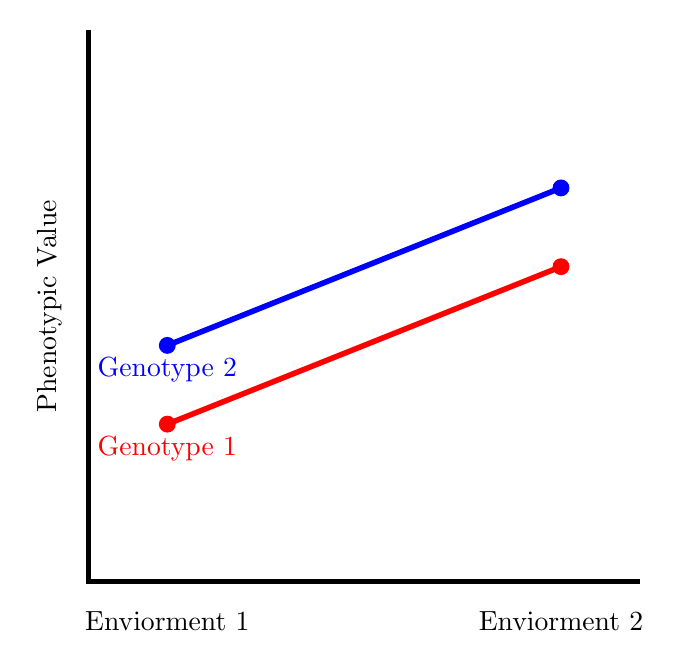
\begin{tikzpicture}
	% axes
	\draw[line width=2, black] (7,0)  -- (0,0) --(0,7);

	% interaction
	\draw[line width=2, red] (1,2) node[below] {Genotype 1}-- (6,4);
	\draw[red, fill=red] (1,2) circle (0.1cm);
	\draw[red, fill=red] (6,4) circle (0.1cm);

	\draw[line width=2, blue] (1,3) node[below] {Genotype 2}-- (6,5);
	\draw[blue, fill=blue] (1,3) circle (0.1cm);
	\draw[blue, fill=blue] (6,5) circle (0.1cm);

	% text
	\node at (1,-0.5) {Enviorment 1};
	\node at (6,-0.5) {Enviorment 2};
	\node[rotate=90] at (-0.5,3.5) {Phenotypic Value};
\end{tikzpicture}
}
        \scalebox{0.5}{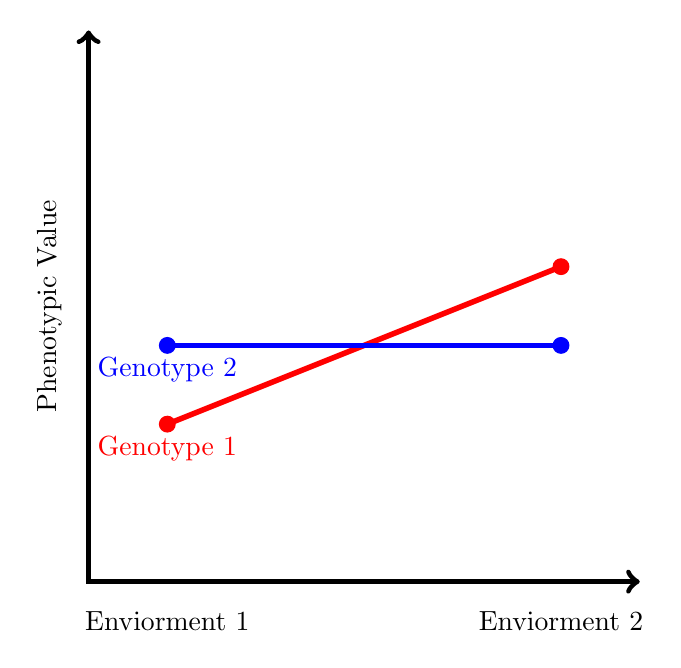
\begin{tikzpicture}
	% axes
	\draw[line width=2, black, <->] (7,0)  -- (0,0) --(0,7);

	% interaction
	\draw[line width=2, red] (1,2) node[below] {Genotype 1}-- (6,4);
	\draw[red, fill=red] (1,2) circle (0.1cm);
	\draw[red, fill=red] (6,4) circle (0.1cm);

	\draw[line width=2, blue] (1,3) node[below] {Genotype 2}-- (6,3);
	\draw[blue, fill=blue] (1,3) circle (0.1cm);
	\draw[blue, fill=blue] (6,3) circle (0.1cm);

	% text
	\node at (1,-0.5) {Enviorment 1};
	\node at (6,-0.5) {Enviorment 2};
	\node[rotate=90] at (-0.5,3.5) {Phenotypic Value};
\end{tikzpicture}
}
      \end{column}
      \begin{column}{0.7\textwidth}
        \begin{center}
          Heritability: 50\%-80\%~\cite{Porsch2016}
        \end{center}
        \begin{itemize}
          \item no genome-wide significant signal~\cite{Vassos2014}
          \item strong phenotypical heterogeneity, low sample size 
          \item gene based analysis suggest \textit{AVPRI1A} 
          \item gene-environment interaction: \textit{MAOA}
        \end{itemize}
      \end{column}
    \end{columns}
    
  \end{frame}

  \section{Longitudinal Heritability of Childhood Aggression}

  \begin{frame}[t]{Sample and Methods}
    \begin{columns}
      \begin{column}{0.5\textwidth}
        \textbf{The Netherlands Twin Register (NTR):}\\
        \begin{itemize}
          \item ages 7, 10 and 12
          \item Child Behavior Checklist (CBCL)
          \item 10,765 twin pairs
        \end{itemize}
      \end{column}
      \begin{column}{0.5\textwidth}
        \textbf{Twin Early Development study (TEDS):}\\
        \begin{itemize}
          \item ages 7, 9 and 12
          \item Strength and Difficulties Questionnaire (SDQ)
          \item 6,897 twin pairs
        \end{itemize}
      \end{column}
    \end{columns}
    \begin{center}
      \scalebox{0.5}{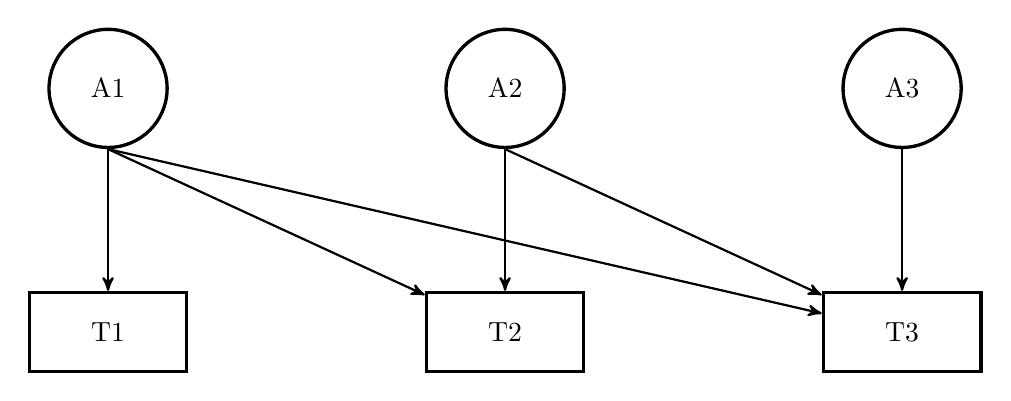
\begin{tikzpicture}[auto,node distance=.5cm,
    latent/.style={circle,draw,very thick,inner sep=0pt,minimum size=15mm,align=center},
    error/.style={circle,draw=none,thin,inner sep=0pt,minimum size=3mm,align=center},
    manifest/.style={rectangle,draw,very thick,inner sep=0pt,minimum width=20mm,minimum height=10mm},
    paths/.style={->, thick, >=stealth'},
    twopaths2/.style={<->, ultra thick,bend left=90, >=stealth'},
    twopaths1/.style={<->, ultra thick,bend right=90, >=stealth'},
    mean/.style={draw, regular polygon, regular polygon sides=3, node distance=1cm, minimum height=3mm, inner sep=0pt}
]

% Define observed variables
\node [latent] (A2) at (0,0) {A2};
\node [latent] (A1) [left=3.5cm of A2] {A1};
\node [latent] (A3) [right=3.5cm of A2] {A3};

\node [manifest] (T1) [below=1.8cm of A1] {T1};
\node [manifest] (T2) [below=1.8cm of A2] {T2};
\node [manifest] (T3) [below=1.8cm of A3] {T3};

\draw [paths] (A1.south) to node {} (T1);
\draw [paths] (A2.south) to node {} (T2);
\draw [paths] (A3.south) to node {} (T3);

\draw [paths] (A1.south) to node {} (T2);
\draw [paths] (A1.south) to node {} (T3);
\draw [paths] (A2.south) to node {} (T3);

\end{tikzpicture}
}
    \end{center}
  \end{frame}

  \begin{frame}[t]{Results}
    \begin{columns}
      \begin{column}{0.5\textwidth}
    \begin{center}
      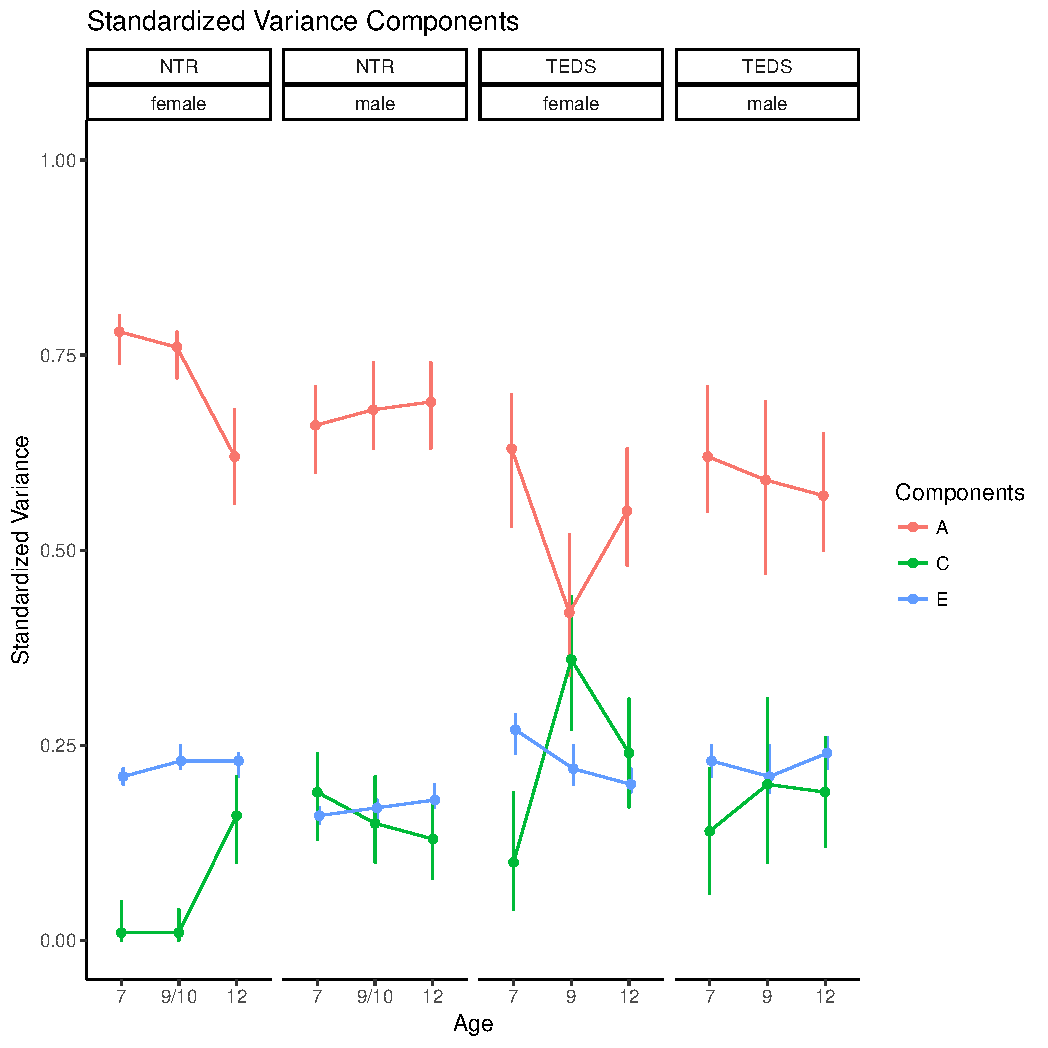
\includegraphics[width=1\linewidth]{plots/varianceComponents.pdf}
    \end{center}
      \end{column}
      \begin{column}{0.5\textwidth}
   \begin{center}
      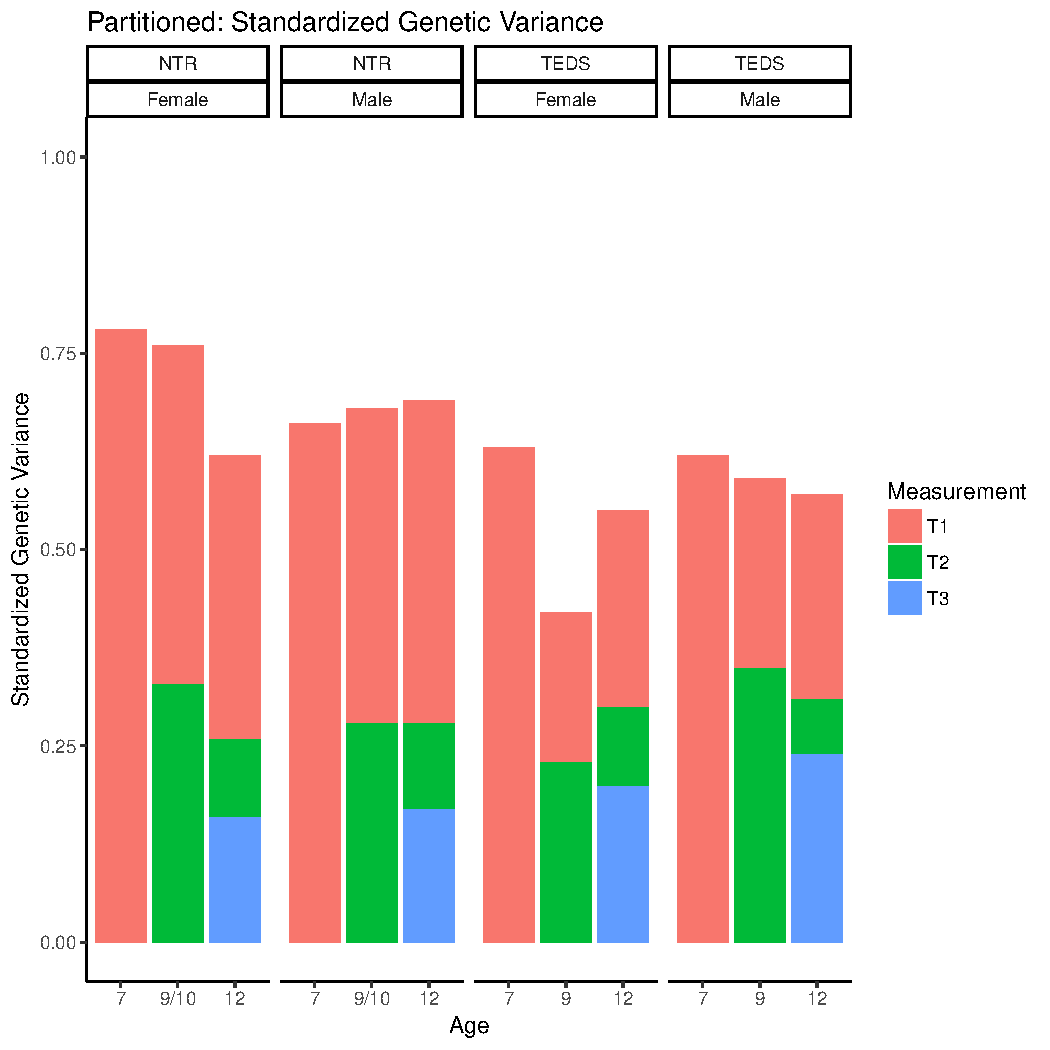
\includegraphics[width=1\linewidth]{plots/partionedGeneticComponents.pdf}
   \end{center} 
      \end{column}
    \end{columns}
    \begin{itemize}
      \item heritability ranges between 42\% and 78\%
      \item genetic factors at T1 are major contributor to the genetic
variance at T2 and T3
      \item genetic contribution of T1 is larger in NTR
    \end{itemize}
  \end{frame}

  \begin{frame}[t]{Stability of Aggression}
    \textbf{High Stability of Genetic Factors:} \\
				Genetic Correlation NTR:\@ $0.76-0.85$ \\
				Genetic Correlation TEDS:\@ $0.64-0.77$ \\
        \vfill
			\adjustbox{max height=\dimexpr\textheight-2.5cm\relax,
				max width=\textwidth}{
				\begin{tabular}{cccc}
	\textbf{NTR}  & \textbf{7 years}  & \textbf{9/10 years} & \textbf{12 years} \\
	7 years       &                   & \cellcolor{blue!25} 0.76 (0.73, 0.78)   &\cellcolor{blue!25} 0.76 (0.72, 0.8) \\
	9/10 years    & \cellcolor{green!25}0.77 (0.72, 0.8)  &                     & \cellcolor{blue!25}0.83 (0.79, 0.88) \\
	12 years      & \cellcolor{green!25}0.77 (0.73, 0.81) & \cellcolor{green!25}0.85 (0.81, 0.89)   & \\
	\textbf{TEDS} & \textbf{7 years}  & \textbf{9 years}    & \textbf{12 years} \\
	7 years       &                   & \cellcolor{blue!25}0.67 (0.57, 0.76)   & \cellcolor{blue!25}0.67 (0.58, 0.75) \\
	9 years       & \cellcolor{green!25}0.64 (0.54, 0.76) &                     & \cellcolor{blue!25}0.77 (0.68, 0.85) \\
	12 years      & \cellcolor{green!25}0.68 (0.6, 0.76)  & \cellcolor{green!25}0.69 (0.61, 0.78)   &
\end{tabular}

			} 
  \end{frame}

  \begin{frame}[t]{Model Comparison}
    \begin{itemize}
      \item Quantitative sex effects present in both studies, although small
        \begin{itemize}
          \item setting parameters to be equal ($NTR: \chi^2_{18}=187.77, P< 0.0001; TEDS: \chi^2_{18}=177.28, P<0.0001$) 
          \item sex specific scalar model  ($NTR: \chi^2_{15}=101.63, P< 0.0001; TEDS: \chi^2_{15}=45.15, P<0.0001$)
        \end{itemize}
      \item Significant effects for common environmental factors
        \begin{itemize}
          \item $NTR: \chi^2_{12}=127.77, P<0.0001; TEDS: \chi^2_{12}=177.28, P<0.0001$
        \end{itemize}
      \item Studies differ significantly
        \begin{itemize}
          \item setting NTR's parameters to be proportional of TEDS's estimate ($\chi^2_{30}=435.07, P< 0.0001$)
        \end{itemize}
    \end{itemize}
  \end{frame}

  \begin{frame}[t]{Conclusion}
    \begin{itemize}
      \item Childhood aggression is a stable trait
      \item Genetic factors are the major source of stability
      \item Individual differences can be mostly accounted by genetic factors
      \item Significant sex differences (mostly common environment), although of small effect
      \item Shared environmental influence are present, especially in boys
      \item Absence of large sex differences is good news for large scale GWAS
    \end{itemize}	
  \end{frame}

  \section{GWASs on Aggression and Risk Taking}

  \begin{frame}[t]{Samples and Phenotype}
    \small
        \textbf{Impulsive Aggression:}
        \begin{displayquote}
          Have you ever had a period of time lasting at least two days when you were so irritable that you found yourself shouting at people or starting fights or arguments?
        \end{displayquote}
        \textbf{Risk Taking:}
        \begin{displayquote}
          Would you describe yourself as someone who takes risks?
        \end{displayquote}
        \resizebox{\textwidth}{!}{%latex.default(samples, title = "", cgroup = c.group, n.cgroup = c(2,     2), table.env = FALSE, file = "./tables/descriptive.tex",     digits = 2)%
\begin{tabular}{llrclr}
\hline\hline
\multicolumn{1}{l}{\bfseries }&\multicolumn{2}{c}{\bfseries All Samples}&\multicolumn{1}{c}{\bfseries }&\multicolumn{2}{c}{\bfseries Caucasian Samples}\tabularnewline
\cline{2-3} \cline{5-6}
\multicolumn{1}{l}{}&\multicolumn{1}{c}{Unaffected/Affected}&\multicolumn{1}{c}{Missingness (in \%)}&\multicolumn{1}{c}{}&\multicolumn{1}{c}{Unaffected/Affected}&\multicolumn{1}{c}{Missingness (in \%)}\tabularnewline
\hline
Risk Taking&107011/39436&$ 3.81$&&86552/29703&$ 3.351$\tabularnewline
Neuroticism&122511&$19.53$&&98086&$18.456$\tabularnewline
Smoking&80984/70678&$ 0.39$&&64115/55853&$ 0.264$\tabularnewline
Impulsive Aggression&40861/9397&$66.99$&&31513/6998&$67.984$\tabularnewline
Drinking&151985&$ 0.17$&&120208&$ 0.065$\tabularnewline
\hline
\end{tabular}
}
  \end{frame}

  \begin{frame}[t]{Phenotype}
    \begin{center}

      \begin{columns}
        \begin{column}{0.5\textwidth}
          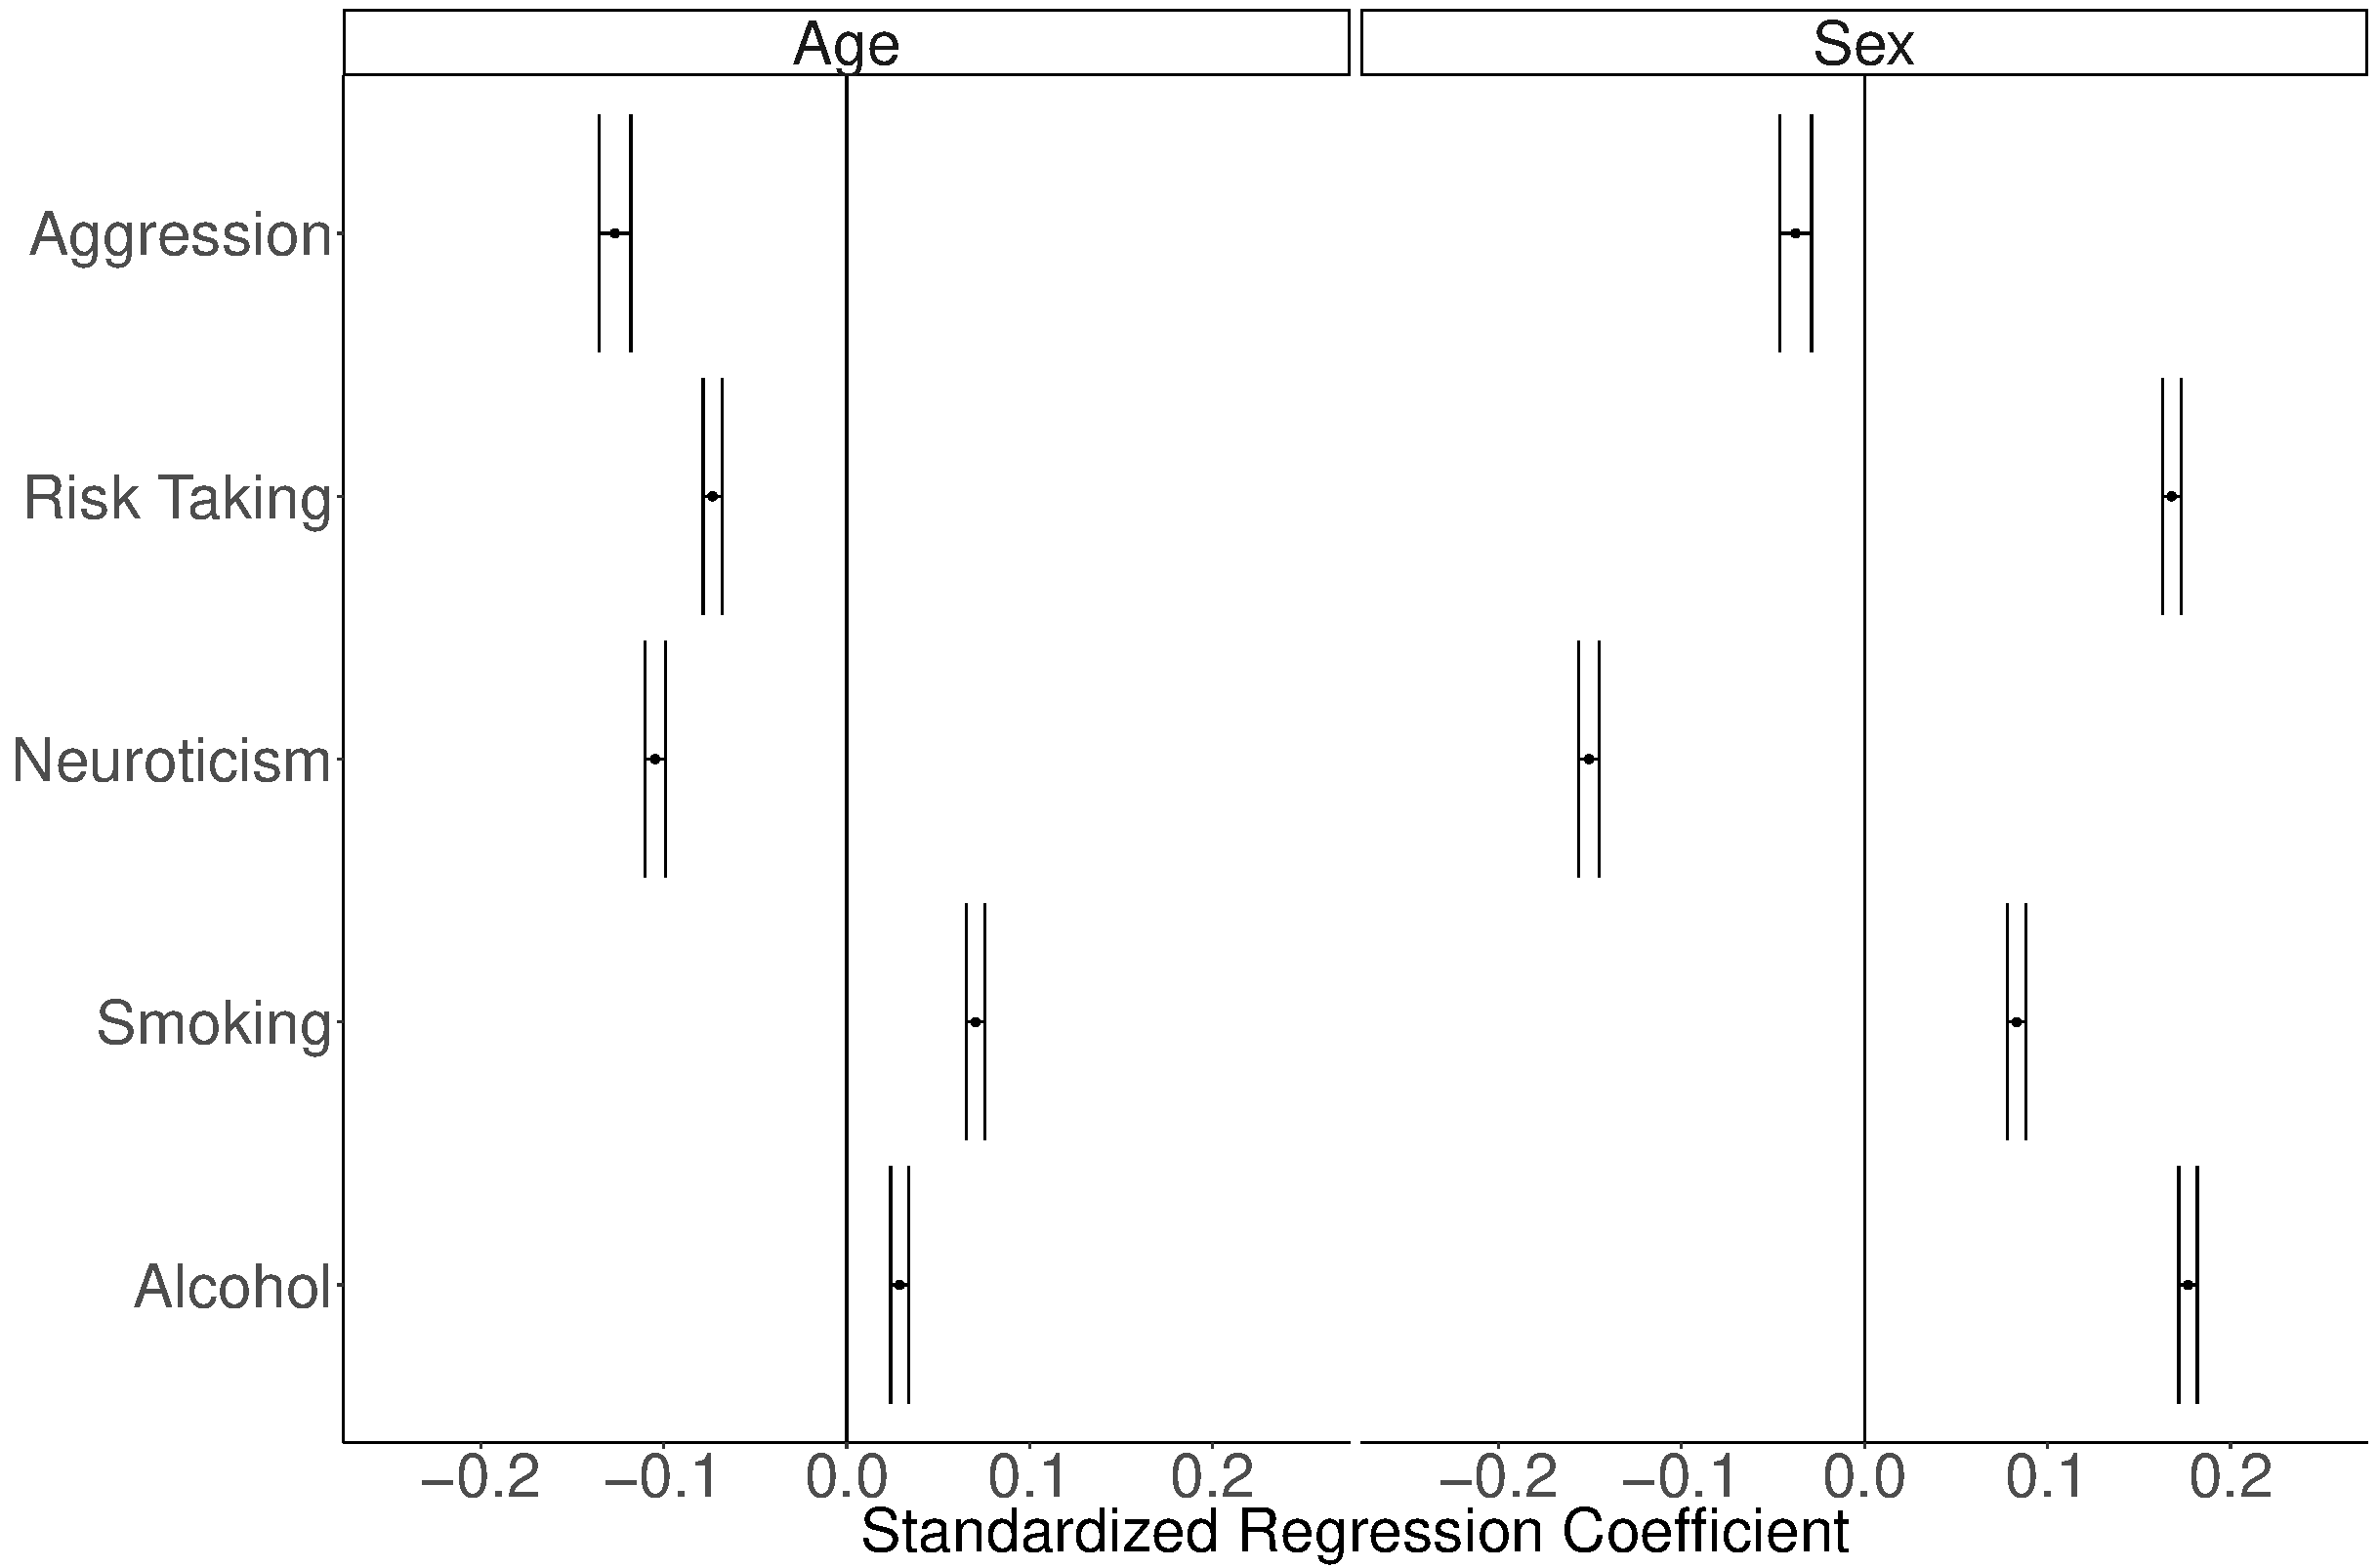
\includegraphics[width=1\linewidth]{../ukb_assoc/figure/phenotype/descriptives_plots.pdf}
        \end{column}
        \begin{column}{0.5\textwidth}
          \begin{itemize}
            {\small
            \item (A) Standardized effect of sex (male=positive, female=negative) on phenotypes. 
            \item (B) Standardized effect of age on phenotypes.
            \item (C) Barplot of neuroticism.
            \item (D) Barplot of alcohol intake.
            }
        \end{itemize}
      \end{column}
    \end{columns}
  \end{center}
\end{frame}

\begin{frame}[t]{Phenotypic Correlation}
  \begin{center}
  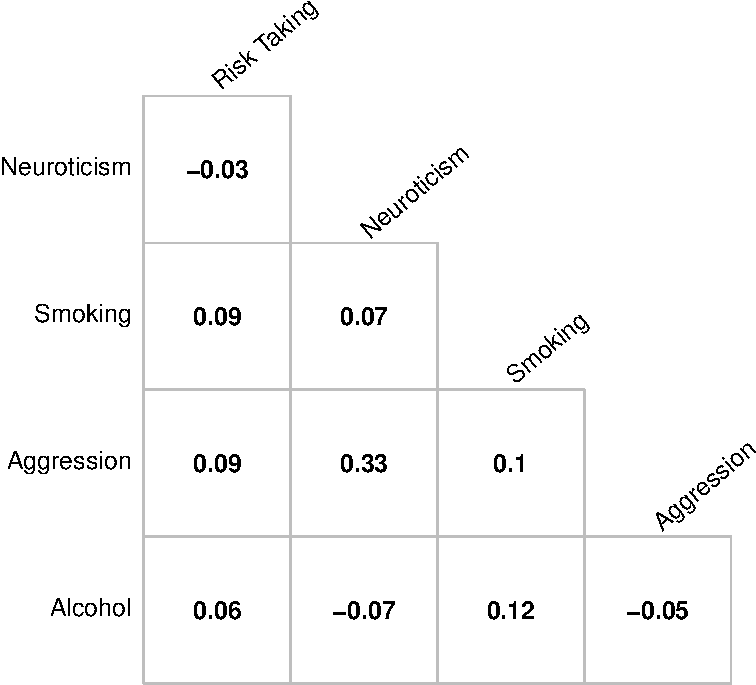
\includegraphics[width=0.6\linewidth]{../ukb_assoc/figure/phenotype/corr_plot_ci.pdf} 
  \end{center}
\end{frame}

  \subsection{Associations}

  \begin{frame}[t]{Genetic Factors}
    \tiny
    \begin{columns}
      \begin{column}{0.6\textwidth}
        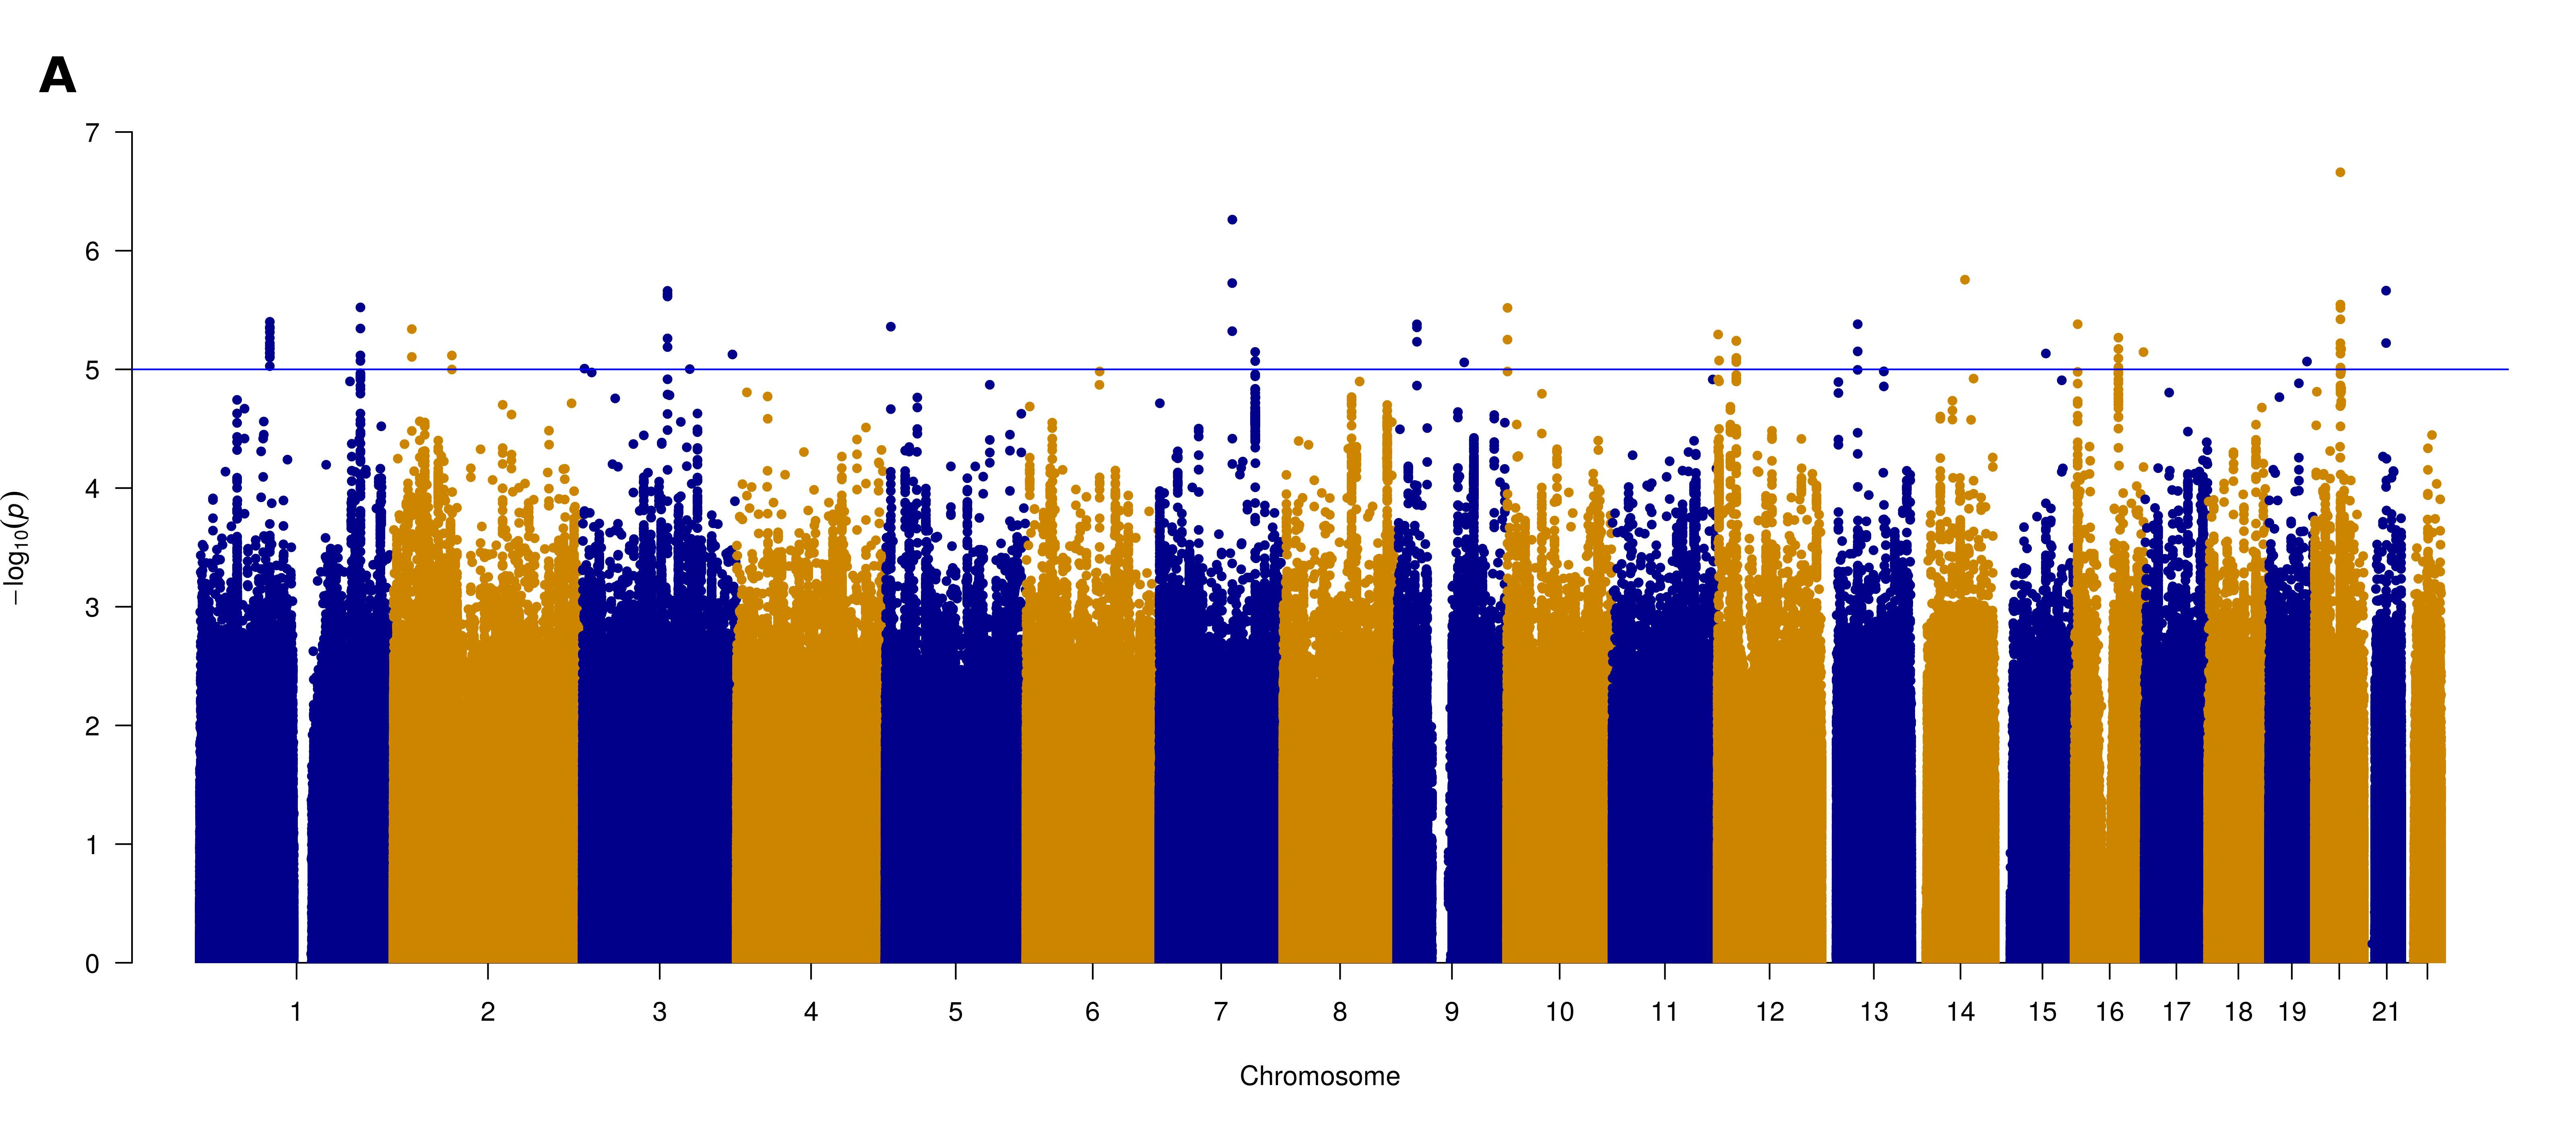
\includegraphics[width=1\linewidth]{../ukb_assoc/figure/manhatten_plots/agg_manhatten_color_2_A.jpeg} \\
        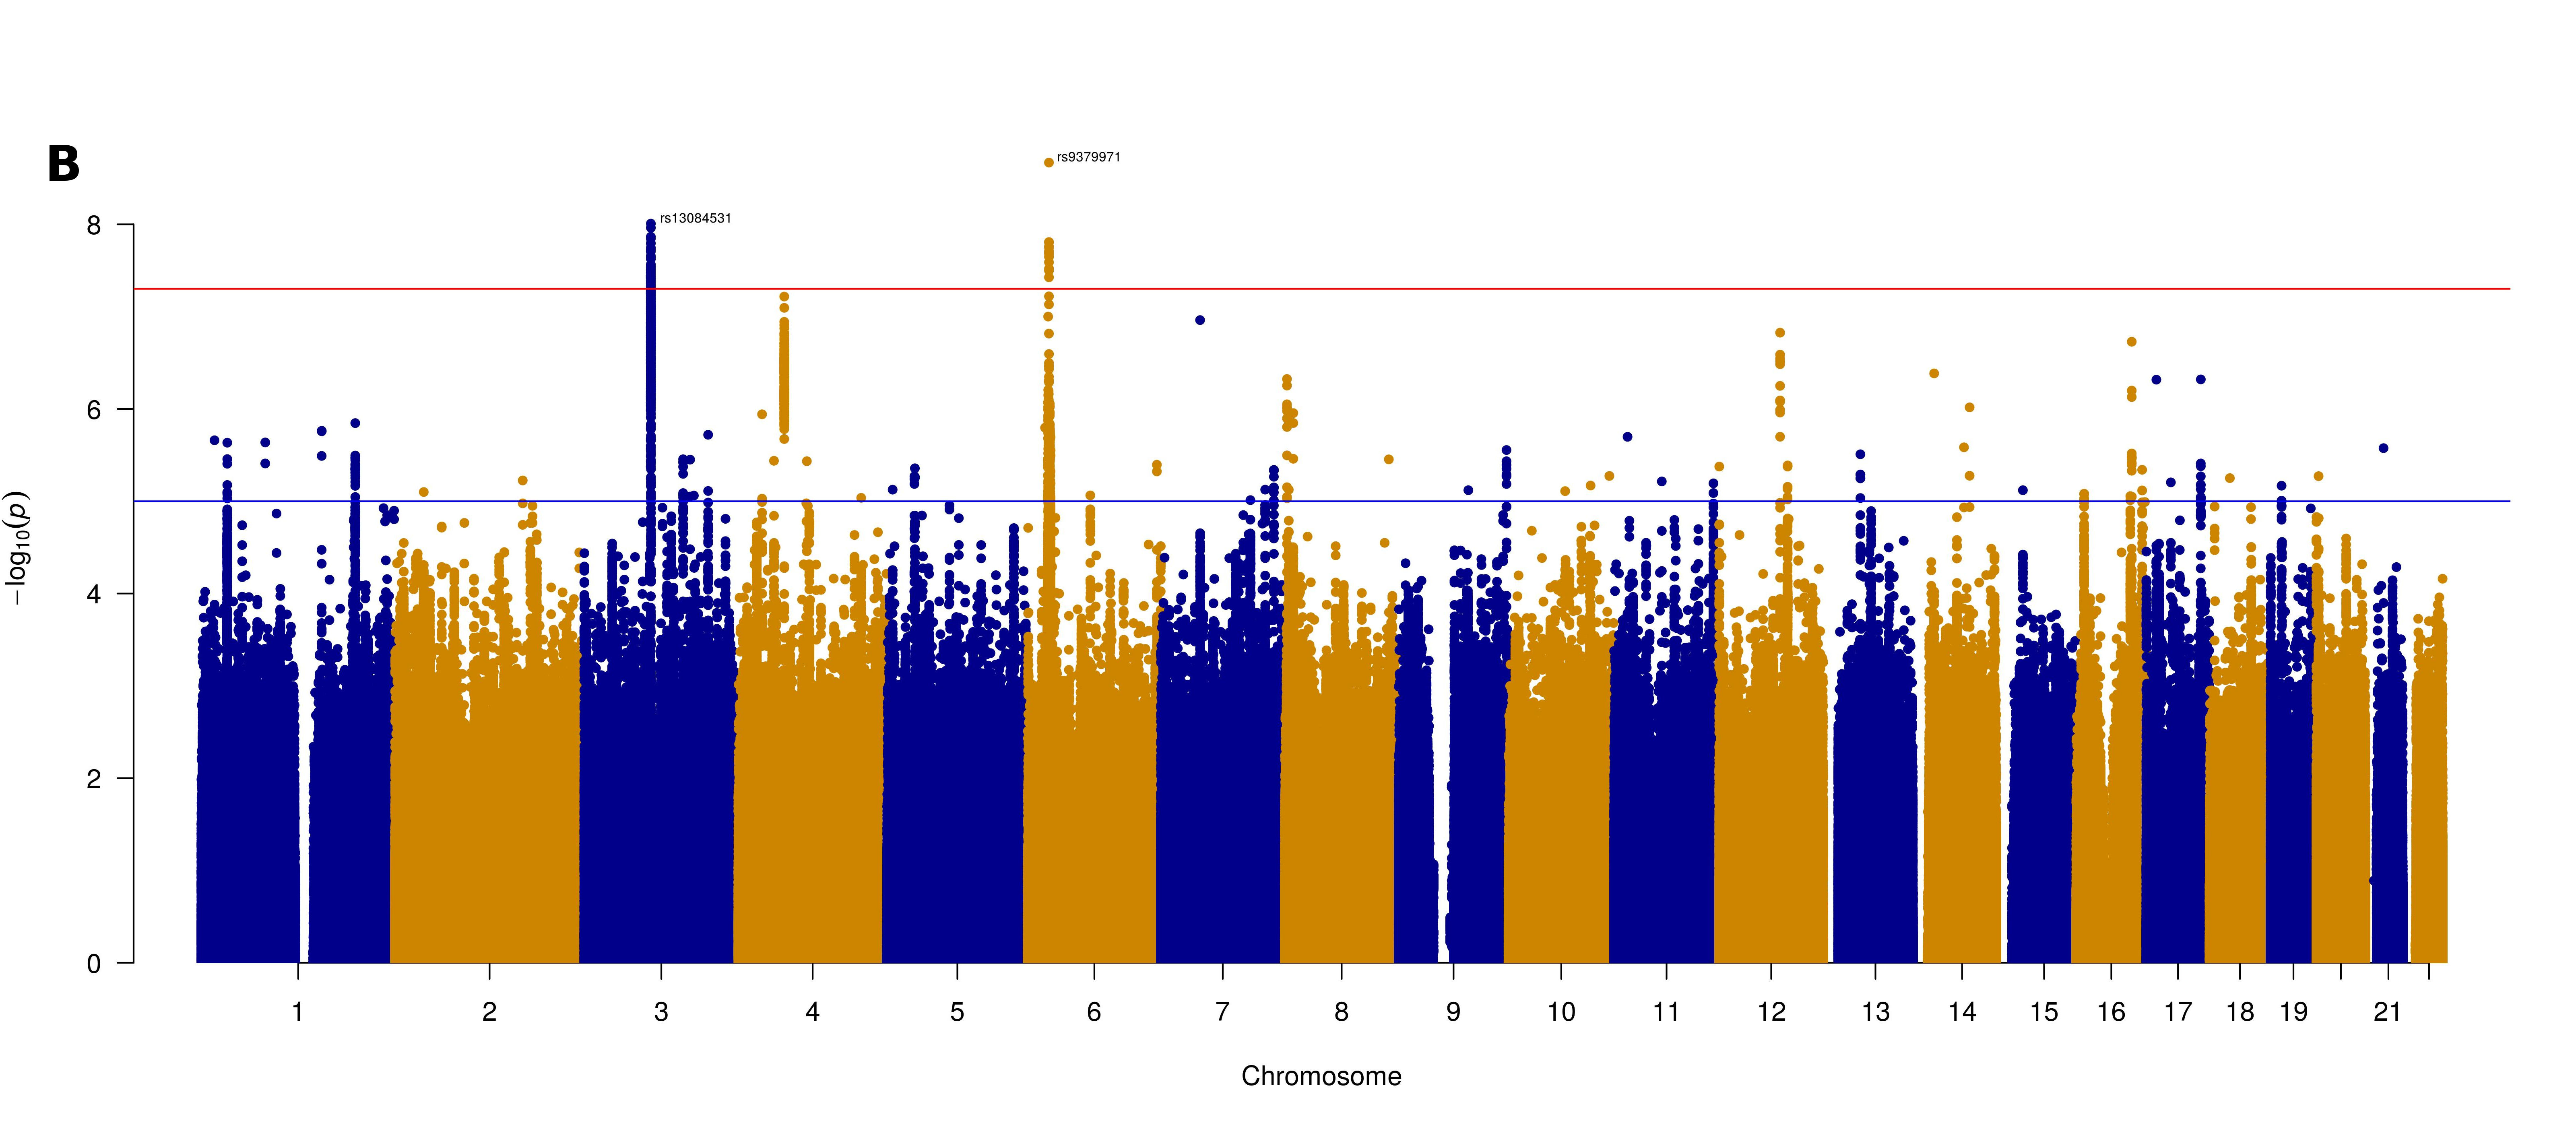
\includegraphics[width=1\linewidth]{../ukb_assoc/figure/manhatten_plots/risk_manhatten_color_B.jpeg}\\
        {\tiny
          (A) Impulsive Aggression;
          (B) Risk Taking
        }
        \begin{itemize}
          \item \textbf{no} genome-wide significant signal in aggression
          \item \textbf{two} genome-wide signals in risk taking
          \item replicating previous findings~\cite{}
        \end{itemize}
        \resizebox{\textwidth}{!}{%latex.default(dat, title = "", file = paste0(outputfolder, "lead_snp_",     nameID, ".tex"), digits = 3, rowname = NULL, table.env = F)%
\begin{tabular}{rlrlrrrr}
\hline\hline
\multicolumn{1}{c}{CHR}&\multicolumn{1}{c}{SNP}&\multicolumn{1}{c}{BP}&\multicolumn{1}{c}{A1}&\multicolumn{1}{c}{N}&\multicolumn{1}{c}{OR}&\multicolumn{1}{c}{STAT}&\multicolumn{1}{c}{P}\tabularnewline
\hline
$3$ & rs13084531 & $85553994$ & G & $115264$ & $0.936$ & $5.73$ & $9.83e-09$\tabularnewline
$6$ & rs9379971  & $27259308$ & T & $109344$ & $1.065$ & $ 5.99$ & $2.14e-09$\tabularnewline
\hline
\end{tabular}
}
      \end{column}
      \begin{column}{0.4\textwidth}
        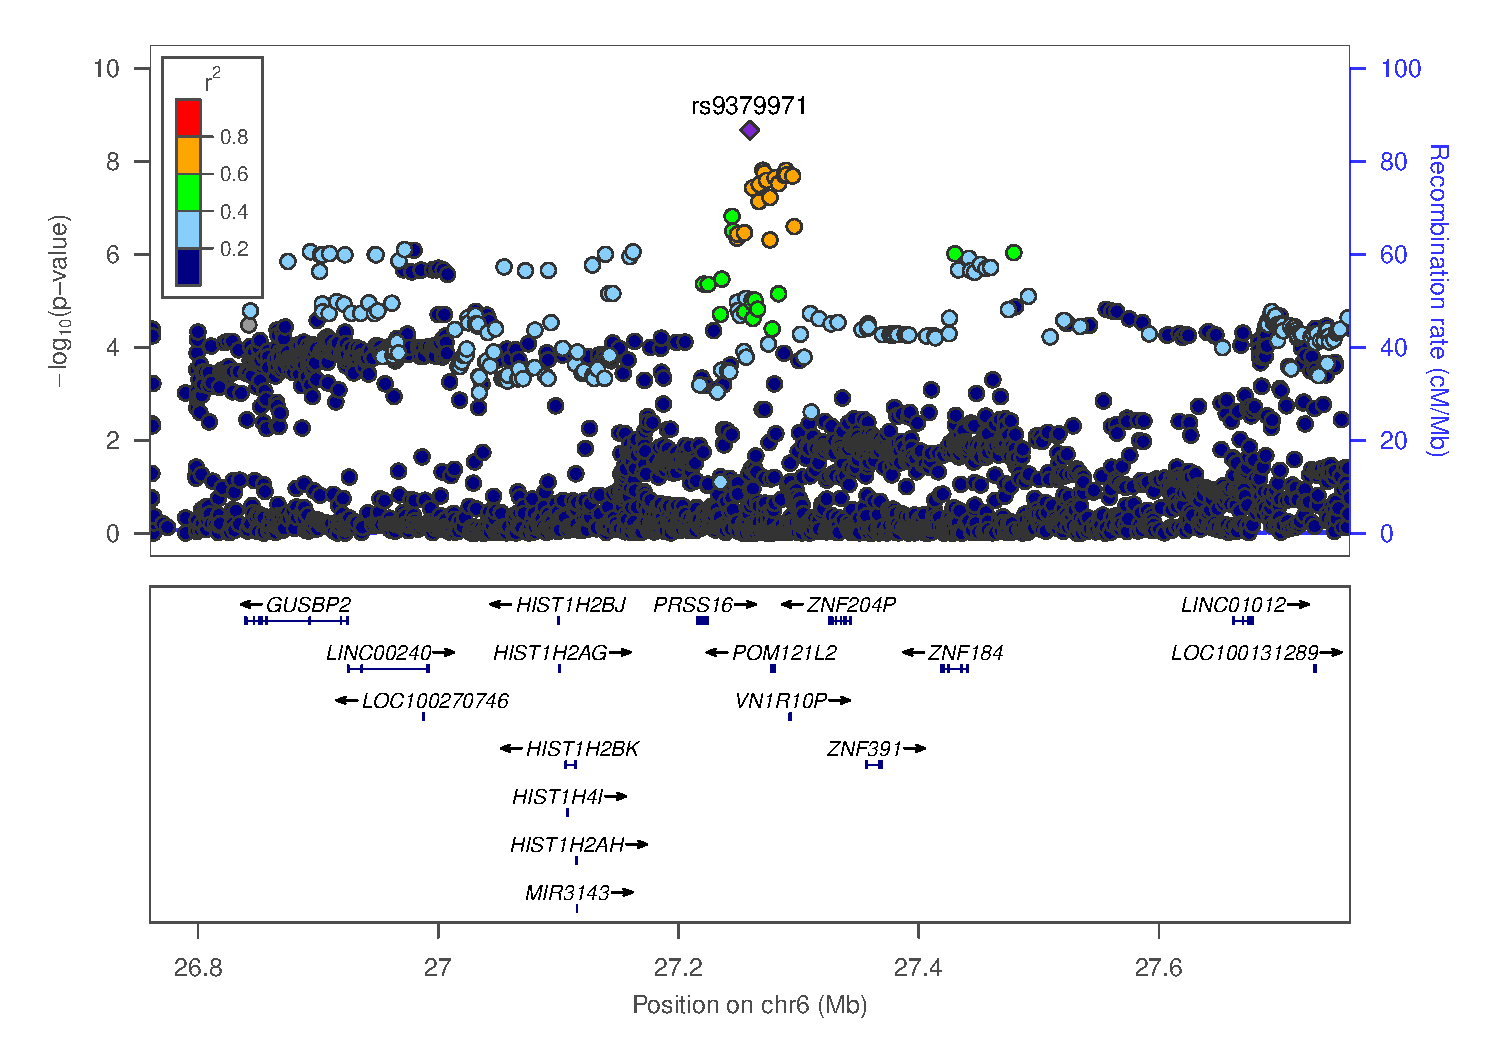
\includegraphics[width=0.8\linewidth, page=1]{{../ukb_assoc/figure/locuszoom/chr6_26759903-27759115}.pdf} \\
        \textbf{rs9379971}\\
        intronic variant with no known phenotypical association
        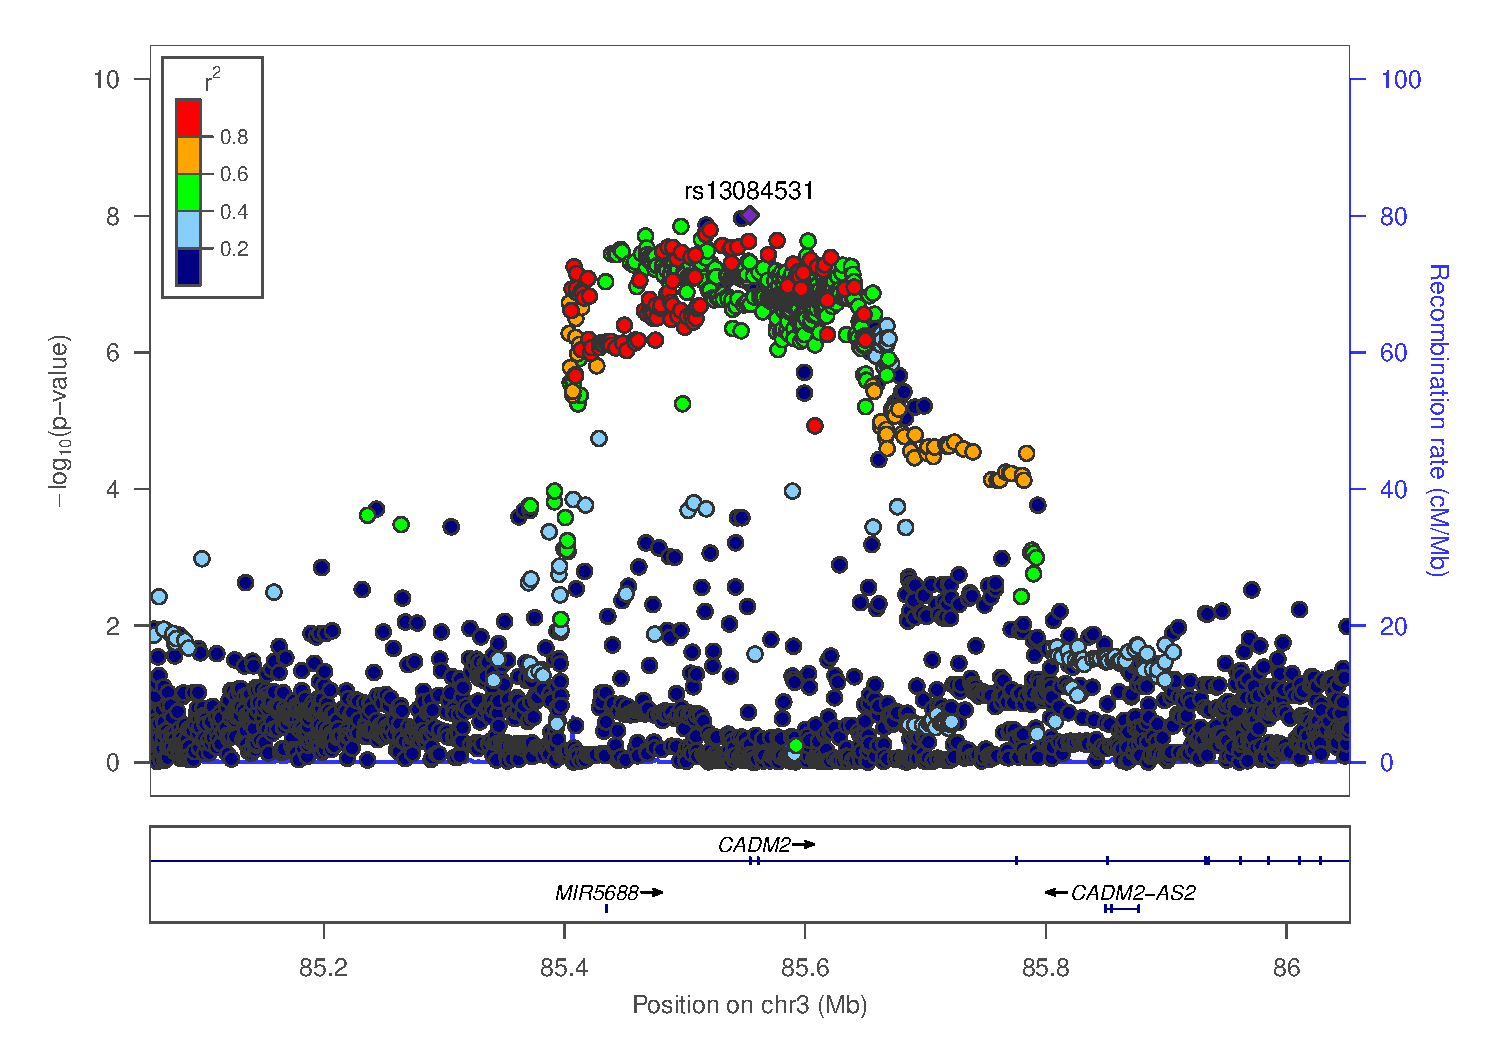
\includegraphics[width=0.8\linewidth, page=1]{{../ukb_assoc/figure/locuszoom/chr3_85055567-86052757}.pdf} \\
        \textbf{rs13084531}\\
        intronic variant related to \textit{CADM2}; previously associated with executive functions
      \end{column}
    \end{columns}
    %\resizebox{\textwidth}{!}{%latex.default(dat, title = "", file = "risk_cFDR.tex", cellTexCmds = cell.format,     numeric.dollar = FALSE, digits = 3, rowname = NULL, table.env = F)%
\begin{center}
\begin{tabular}{rlrrlllr}
\hline\hline
\multicolumn{1}{c}{CHR}&\multicolumn{1}{c}{SNP}&\multicolumn{1}{c}{cFDR}&\multicolumn{1}{c}{Z}&\multicolumn{1}{c}{A1}&\multicolumn{1}{c}{A2}&\multicolumn{1}{c}{$\delta$}&\multicolumn{1}{c}{$Z_{\delta}$}\tabularnewline
\hline
    1&   rs1912231&   5.25e-03&    4.34&   C&   T&   Alcohol&    3.62\tabularnewline
    3&   rs9870448&   2.77e-04&   -5.24&   A&   G&   Alcohol&   -3.89\tabularnewline
\bfseries    3&\bfseries   rs570682061&\bfseries   6.64e-05&\bfseries    5.22&\bfseries   A&\bfseries   AT&\bfseries   Smoking&\bfseries    3.67\tabularnewline
    6&   rs7744605&   7.52e-05&    5.16&   C&   A&   Smoking&    3.27\tabularnewline
    6&   rs9468372&   2.06e-04&    4.88&   T&   A&   Smoking&    3.42\tabularnewline
    8&   rs1968400&   9.86e-03&    3.67&   G&   C&   Smoking&    3.23\tabularnewline
    8&   rs116807689&   2.62e-03&    4.16&   A&   G&   Smoking&    3.73\tabularnewline
   10&   rs67657945&   2.13e-03&   -4.23&   CT&   C&   Smoking&   -3.21\tabularnewline
\hline
\end{tabular}\end{center}
}
  \end{frame}

  \subsection{Genetic Correlations}

  \begin{frame}[t]{Conditional False Discovery Rate}
    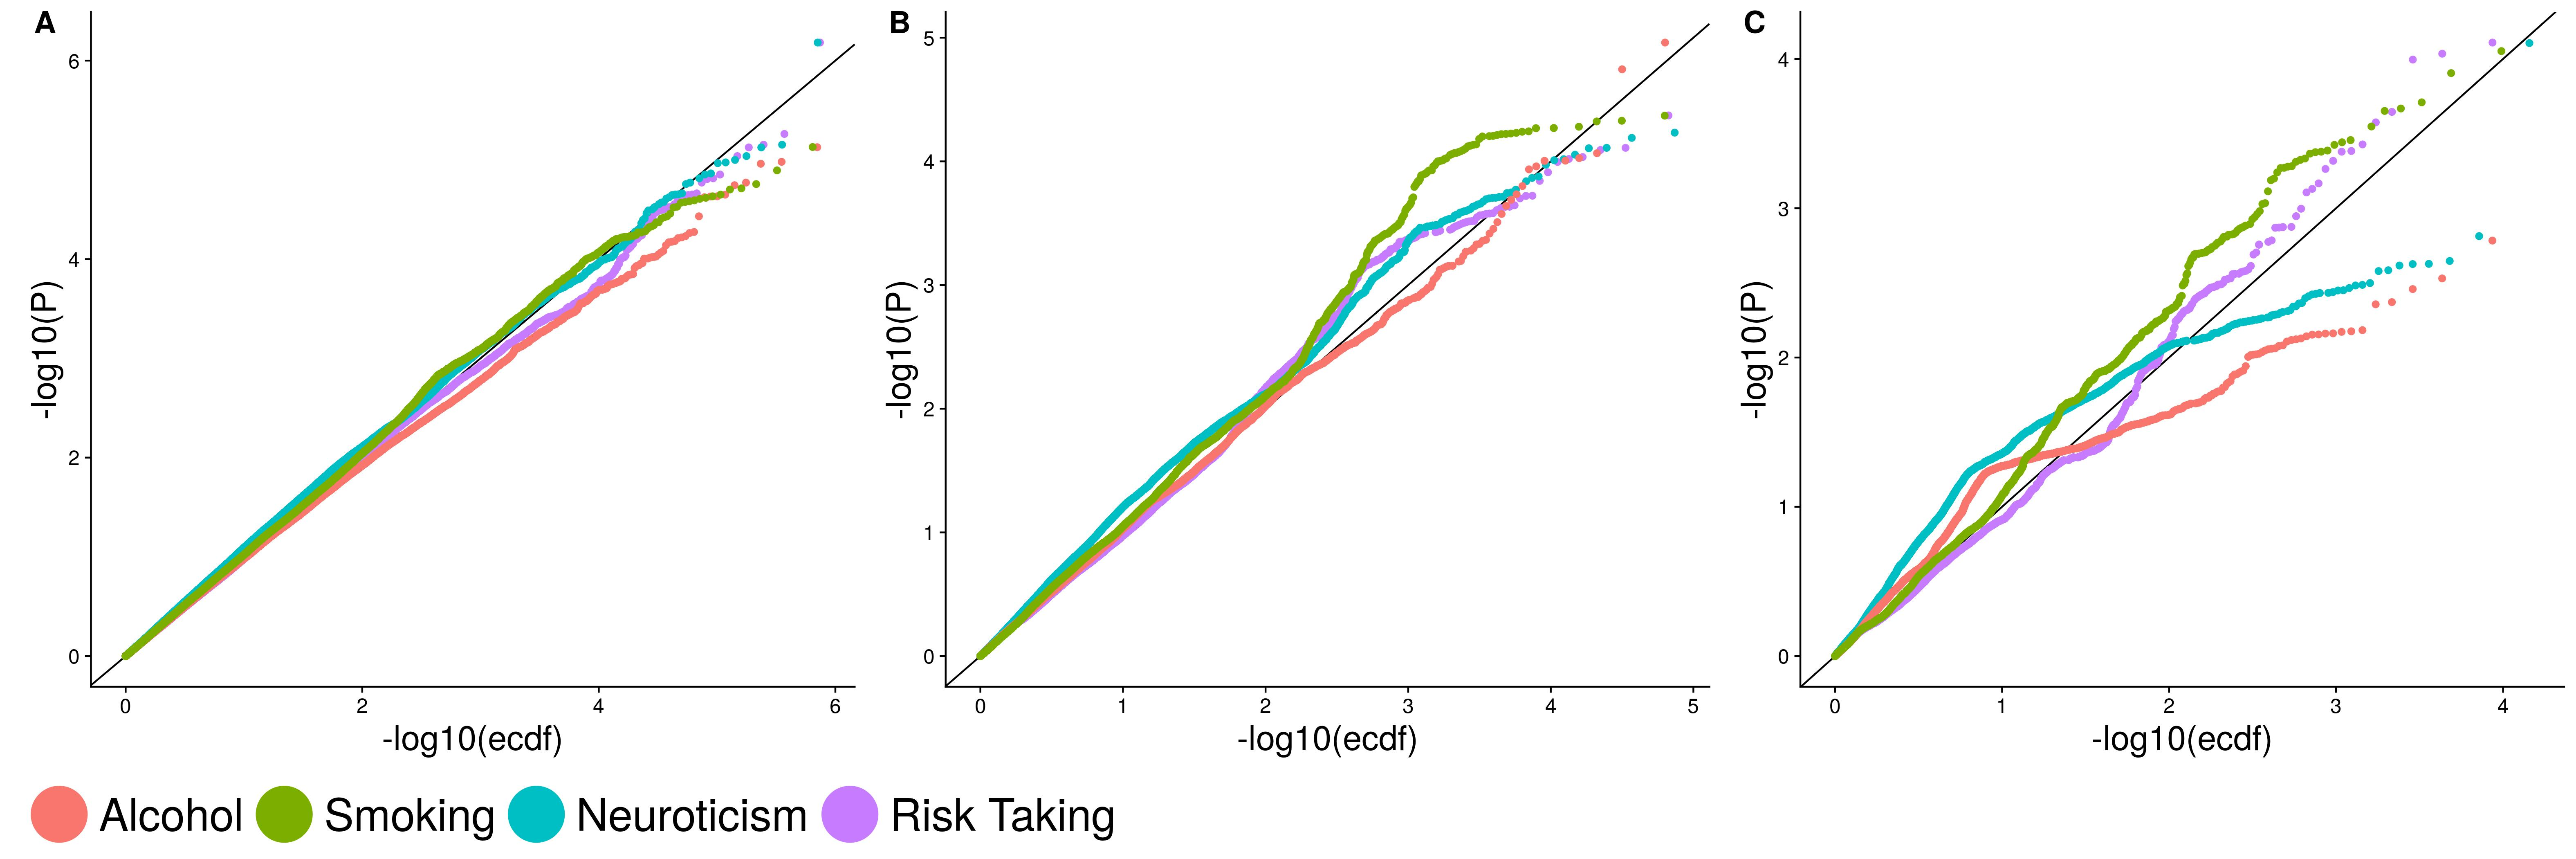
\includegraphics[width=1\linewidth]{../ukb_assoc/figure/cFDR/agg_cond.jpeg} \\
    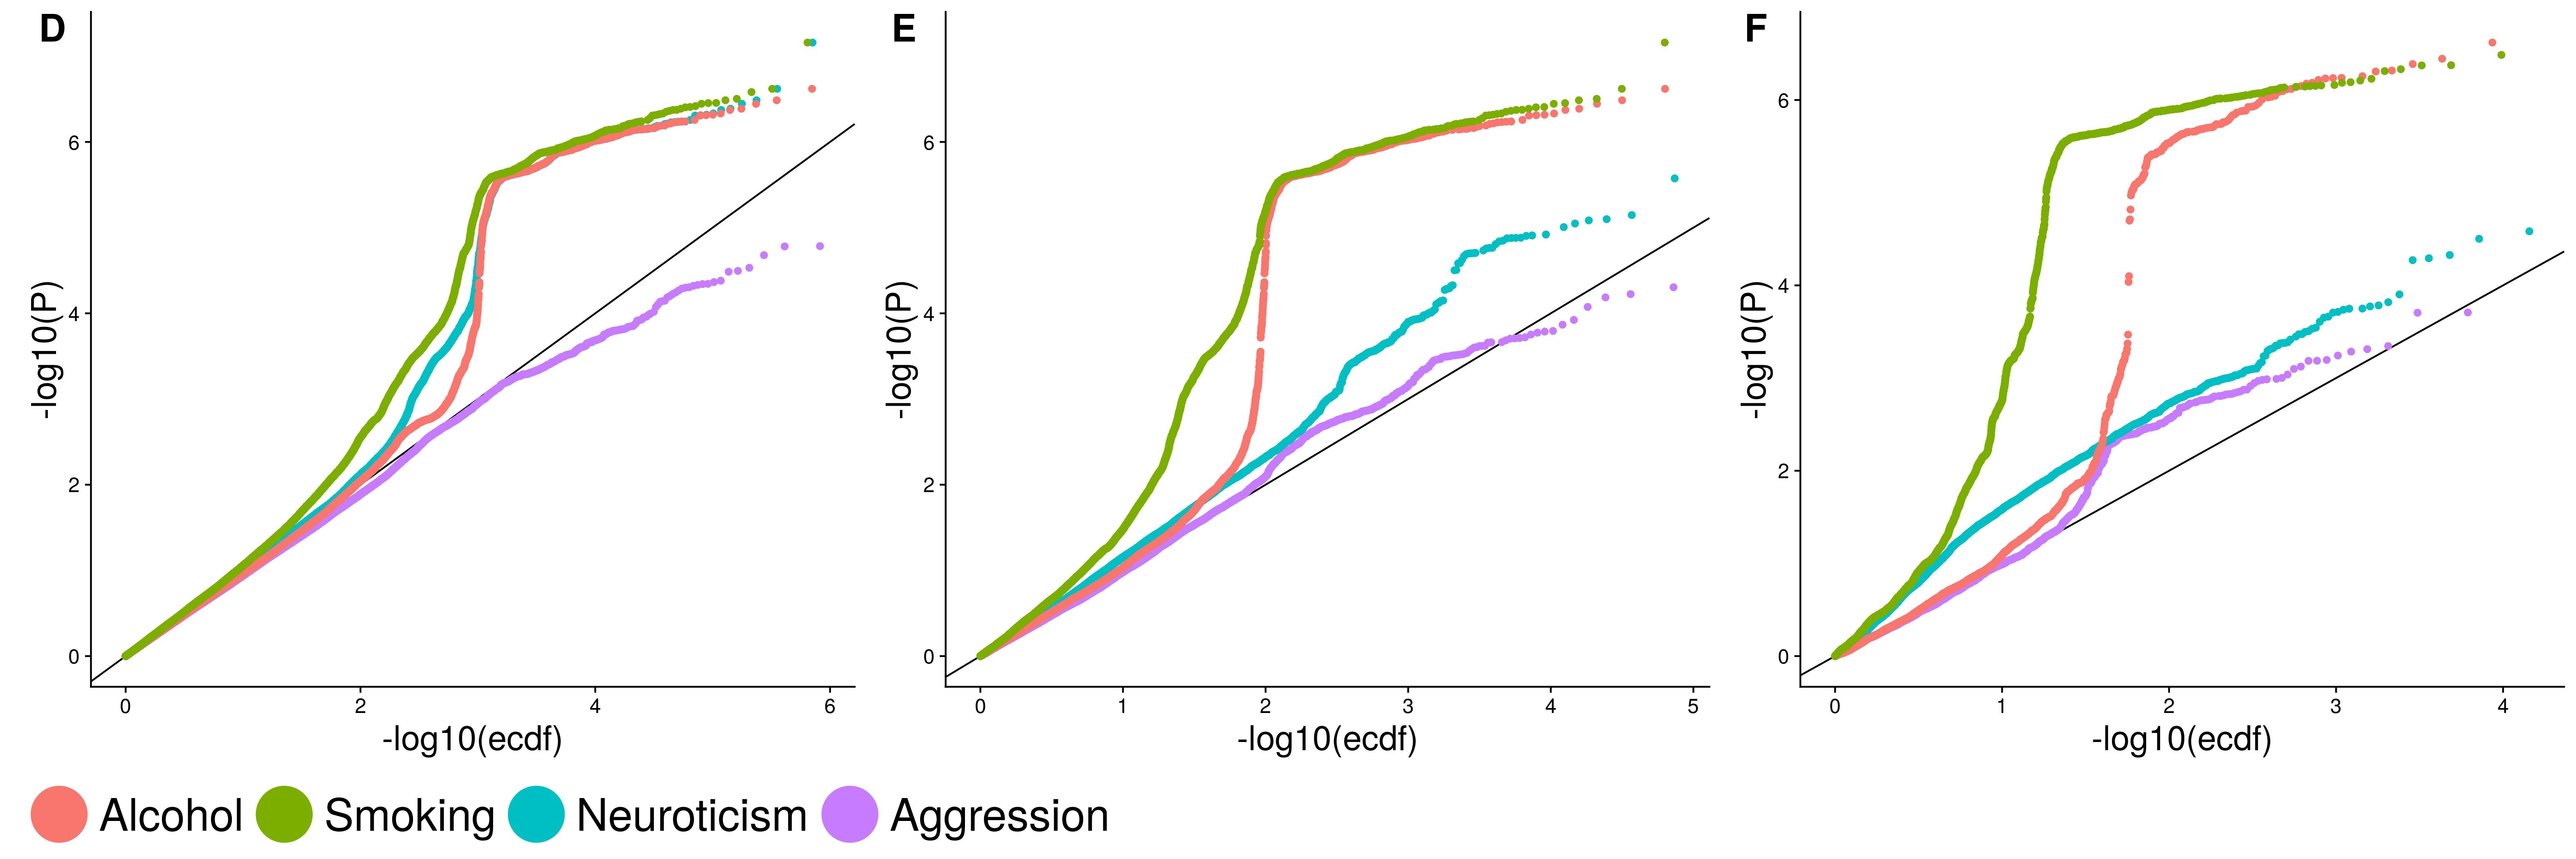
\includegraphics[width=1\linewidth]{../ukb_assoc/figure/cFDR/risk_cond.jpeg}\\
    %Conditional QQ plots for both risk taking and aggression. 
    %Panels A--C present the  QQ-plots for impulsive aggression,
    %conditional on the remaining phenotypes given threshold $p\leq0.1$, $p\leq0.01$, $p\leq0.001$ respectively.
    %Similarly, panels D--F are the  QQ-plots for risk taking, conditional on the remaining phenotypes across the three thresholds
  \end{frame}

  \begin{frame}[t]{Genetic Correlations}
  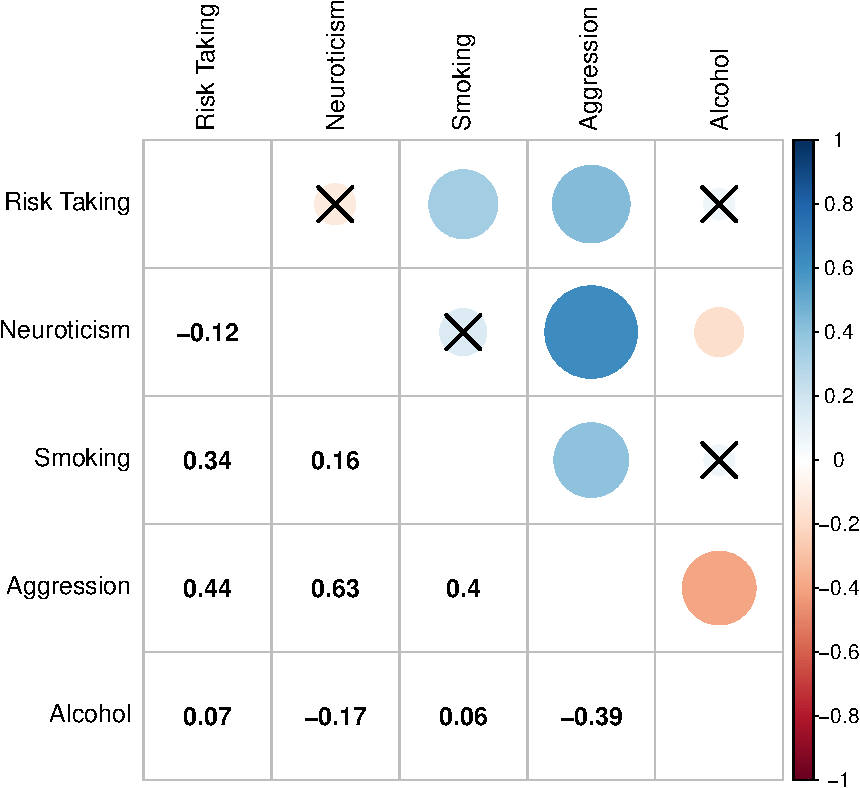
\includegraphics[width=0.8\linewidth]{../ukb_assoc/figure/genetic_corr/gcorr_plot_circle_full_se.pdf}
  \end{frame}

  \begin{frame}[t]{Results}
    
  \end{frame}

  \section{Causal Inference between Aggression and Psychiatric Disorders}

  \begin{frame}[t]{Sample and Methods}
    
  \end{frame}

  \begin{frame}[t]{Results}
    
  \end{frame}

  \section{Distributional Differences of Rare Variants}

  \begin{frame}[t]{Idea and Methods}
    
  \end{frame}

  \begin{frame}[t]{Results and Discussion}
    
  \end{frame}

  \section{Discussion}

  \begin{frame}[t]{Discussion}
    
  \end{frame}
  
  
  
\bibliography{/home/robert/Documents/library.bib}
\end{document}
